
\documentclass[10pt]{beamer}

\usepackage{algpseudocode}

\usetheme{Montpellier}
\usecolortheme{rose}

% page numbers, from
% https://tex.stackexchange.com/questions/137022/how-to-insert-page-number-in-beamer-navigation-symbols
\expandafter\def\expandafter\insertshorttitle\expandafter{%
  \insertshorttitle\hfill%
  \insertframenumber\,/\,\inserttotalframenumber}

\newcommand{\stanza}{ \\~\ }

\title{04. Randomization}
\subtitle{CPSC 535 $\sim$ Fall 2019}
\author{Kevin A. Wortman}
\institute{ 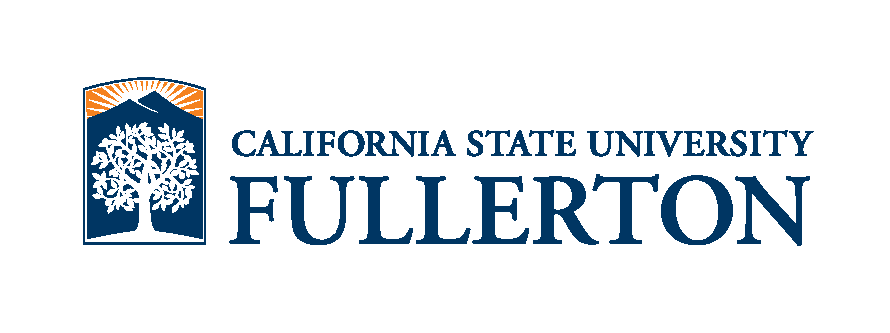
\includegraphics[height=2cm]{csuf-logo-cmyk} }
\date{September 16, 2019 \stanza

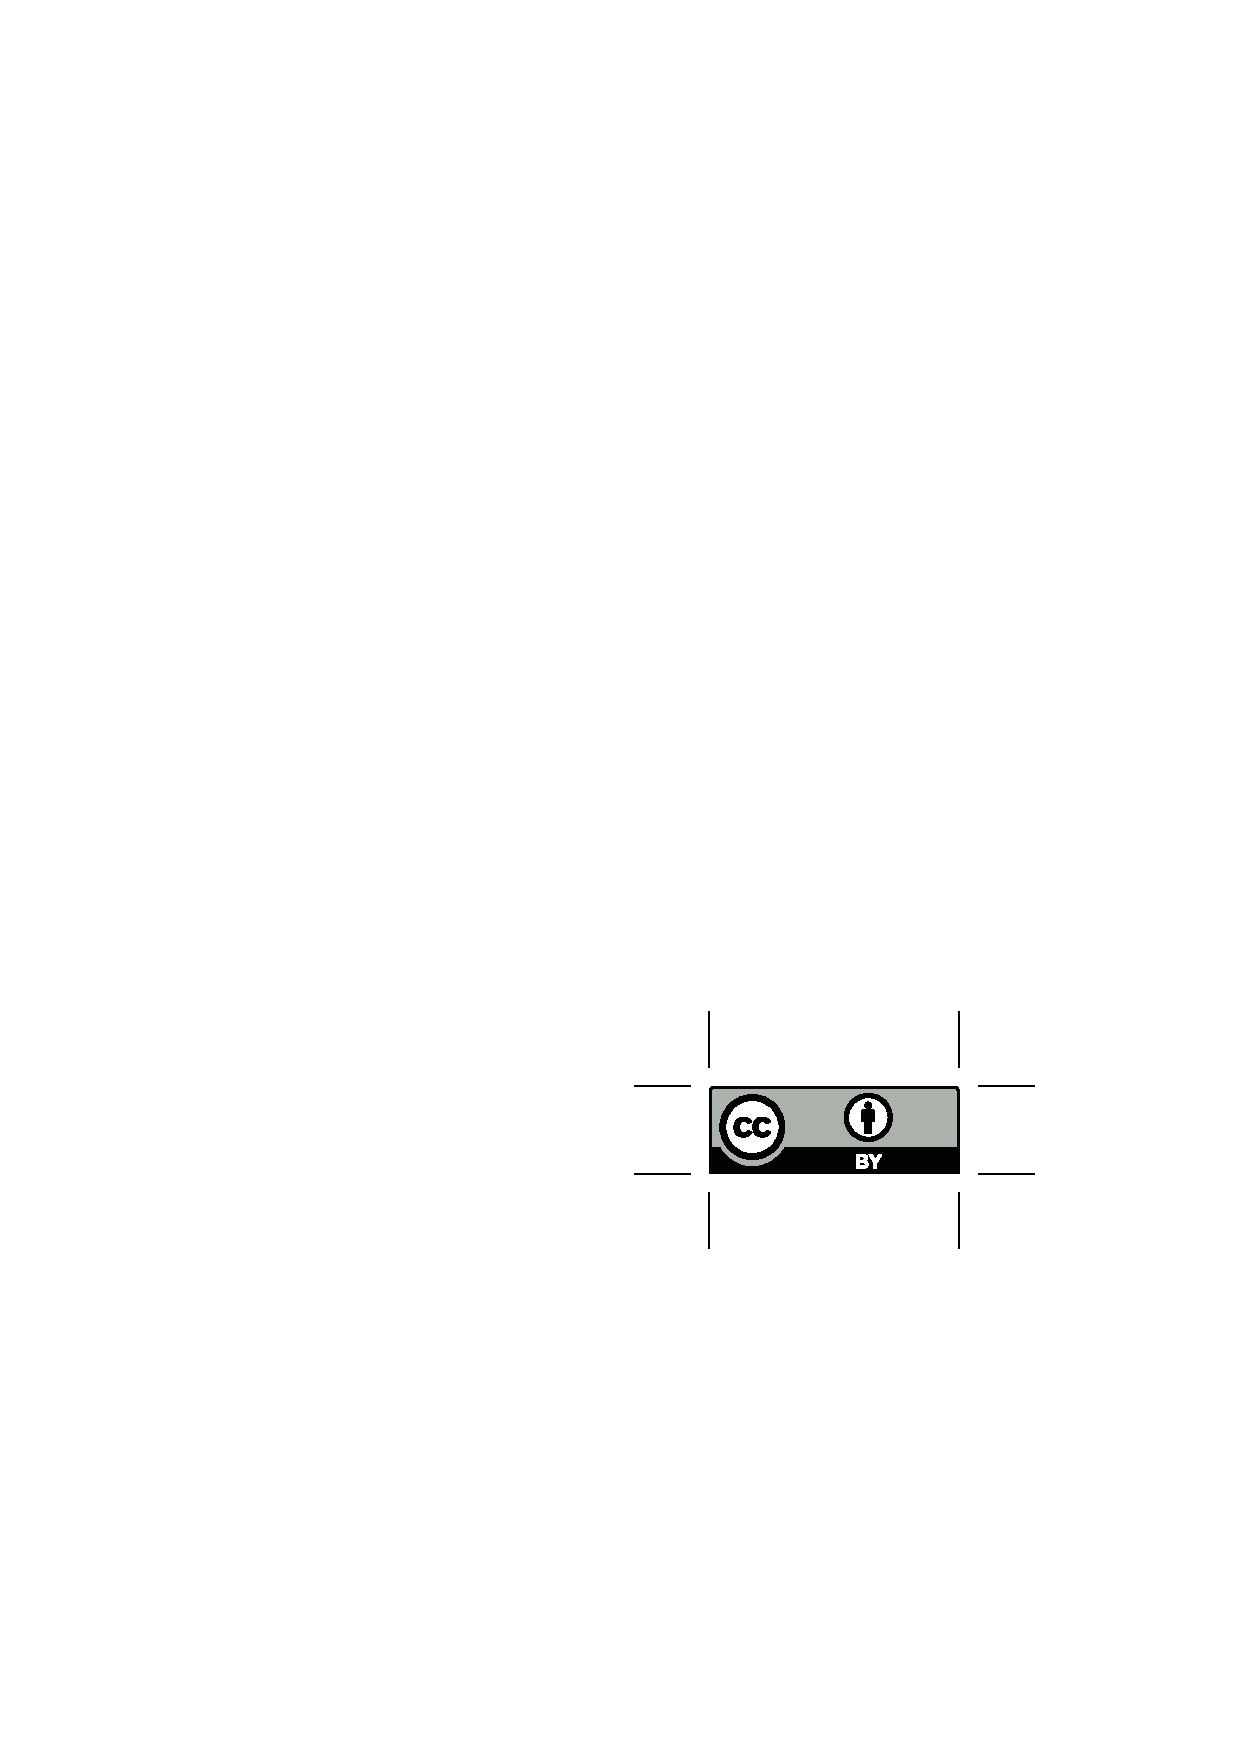
\includegraphics[height=14pt]{by} \\

{\tiny
This work is licensed under a
\href{http://creativecommons.org/licenses/by/4.0/}{Creative Commons Attribution 4.0 International License}.
}}

\begin{document}

\begin{frame}
  \titlepage
\end{frame}

\begin{frame} \frametitle{Randomization}

\emph{Big idea:} a \emph{randomized} algorithm deliberately makes random choices
\begin{itemize}
  \item con: behavior and/or performance becomes \emph{stochastic}
  \item pro: other aspects can get better (speed, simplicity)
  \item often algorithm gets faster/simpler but analysis gets harder
    (recall this is a win)
\end{itemize}

E.g. quicksort, recall
\begin{itemize}
  \item every sorting algorithm takes $\Omega(n \log n)$ time
  \item merge sort takes $\Theta(n \log n)$ worst-case time but $\Theta(n)$
    temporary space
  \item quicksort is randomized, takes $\Theta(n \log n)$ expected time but only
    $\Theta(\log n)$ space \emph{(in-place)}, better constant factors
\end{itemize}
\end{frame}

\begin{frame} \frametitle{Kinds of Time Bounds}
Suppose algorithm $A$ takes...
\begin{itemize}
  \item \underline{$\Theta(n)$ deterministic worst-case time}: for \emph{every} input, $A$ takes $\Theta(n)$ time
  \item \underline{$\Theta(n)$ average time}: the mean time, \emph{averaging over every
    possible input,} is $\Theta(n)$
    \begin{itemize}
      \item only relevant when each input is equally likely
      \item not true for e.g. sorting, maximum subarray
      \item in principle we could take a weighted average, but we'd need to know
        the probability distribution of inputs, unlikely
    \end{itemize}
  \item \underline{$\Theta(n)$ expected time}: the mean time, \emph{averaging over
    every sequence of random choices} $A$ could make, is $\Theta(n)$
    \begin{itemize}
      \item no assumption about input; still assume worst case
    \end{itemize}
  \item by default, ``$\Theta(n)$ time'' means $\Theta(n)$ deterministic worst-case time
\end{itemize}
\end{frame}

\begin{frame} \frametitle{Deterministic versus Randomized Algorithms}
If alg $A$ is \textbf{deterministic}: its deterministic worst-case time
and expected time bound are always the same
\begin{itemize}
  \item technically, we can say linear search takes ``$\Theta(n)$ expected time''
  \item but this is kind of misleading/distracting
\end{itemize}
$A$ \textbf{is randomized}: usually expected-case is faster than worst-case
\begin{itemize}
  \item (because expected-case is an average, worst-case is a maximum)
  \item hash table insert: $\Theta(1)$ expected time, $\Theta(n)$ worst-case time
  \item treap insert: $\Theta(\log n)$ expected time, $\Theta(n)$ worst-case time
  \item quicksort: $\Theta(n \log n)$ expected time, $\Theta(n^2)$ worst-case time
\end{itemize}
\end{frame}

\begin{frame} \frametitle{Multiplying Randomized Bounds}
\begin{itemize}
  \item Multiplying works normally
  \item If running $A$ once takes $O(E)$ expected time and $O(W)$ worst-case time...
  \item ...then running $A$ $(k)$ times takes $O(kE)$ expected time and $O(kW)$ worst-case time.
  \item So
  \begin{itemize}
    \item $k$ hash table inserts takes $O(k)$ expected time and $O(kn)$ worst-case time
    \item $n$ hash table inserts takes $O(n)$ expected time and $O(n^2)$ worst-case time
    \item $n$ treap inserts takes $O(n \log n)$ expected time and $O(n^2)$ worst-case time
  \end{itemize}
\end{itemize}

\end{frame}

\begin{frame} \frametitle{Adding Randomized Bounds}
adding works normally with two caveats
\begin{enumerate}
  \item the \emph{expected} qualifier is ``sticky''
    \begin{itemize}
      \item $O(D)$ worst-case time + $O(E)$ expected time = $O(\max\{D,E\})$ expected-time
      \item $\implies$ insert $n$ elements into hash table, then loop through hash table
        $= O(n) \text{ expected } + O(n) \text{ worst-case } = O(n)$ expected
    \end{itemize}
  \item however, you have the option of using a randomized alg's worst-case bound
    \begin{itemize}
      \item $\implies$ insert $n$ elements into hash table, then sort elements with
        insertion sort
        $ = O(n) \text{ expected } + O(n^2) \text{ worst-case } = O(n^2)$ expected time
      \item but we could also use hash tables' worst-case bound and say
        $= O(n^2) \text{ worst-case } + O(n^2) \text{ worst-case } = O(n^2)$ worst-case
    \end{itemize}
\end{enumerate}

Ordinarily
\begin{itemize}
  \item $O(T)$ worst-case time is better than $O(T)$ expected time
  \item faster expected-time is better than slower worst-case time
\end{itemize}
\end{frame}

\begin{frame} \frametitle{Maximum}
  {\footnotesize
  \begin{algorithmic}[1]
    \Function{MAXIMUM}{$A$}
    \State best $ = $ NIL
    \For { $x$ in $A$ }
      \If { best is still NIL or $x > $ best }
        \State best $= x$
      \EndIf
    \EndFor
    \State \Return { best }
    \EndFunction
  \end{algorithmic}
  }
  \begin{itemize}
  \item (CLRS calls this \emph{hiring,} but it generalizes to any kind of find-the-best process.)
  \item Suppose the ``best $= x$'' step is expensive (e.g. moving your house).
  \item \emph{Q: how many times is best reassigned in the best case?}
  \item \emph{Q: what about the worst case?}
\end{itemize}
\end{frame}

\begin{frame} \frametitle{Maximum (continued)}
  {\footnotesize
  \begin{algorithmic}[1]
    \Function{MAXIMUM}{$A$}
    \State best $ = $ NIL
    \For { $x$ in $A$ }
      \If { best is still NIL or $x > $ best }
        \State best $= x$
      \EndIf
    \EndFor
    \State \Return { best }
    \EndFunction
  \end{algorithmic}
  }
\vspace{.5cm}
A best-case: $A$ in decreasing order; reassigned only once \\
\vspace{.5cm}
A worst-case: $A$ in increasing order; reassigned $n$ times
\end{frame}

\begin{frame} \frametitle{Randomized Maximum}
  {\footnotesize
  \begin{algorithmic}[1]
    \Function{RANDOMIZED-SMAXIMUM}{$A$}
    \State permute $A$ randomly \Comment{only change}
    \State best $ = $ NIL
    \For { $x$ in $A$ }
      \If { best is still NIL or $x > $ best }
        \State best $= x$
      \EndIf
    \EndFor
    \State \Return { best }
    \EndFunction
  \end{algorithmic}
  }
  \begin{itemize}
    \item best-case: luckily visit maximum first, only one reassign
    \item worst-case: unluckily visit in increasing order, reassign $n$ times
    \item (same)
    \item \textbf{but what about the expected number of reassigns?}
  \end{itemize}
\end{frame}

\begin{frame} \frametitle{Randomized Maximum Analysis}
Define
\[ X_i = \{\text{1 if best is reassigned in iteration } i, 0 \text{ otherwise} \} .\]
Observe
\[ X_i = 1 \text{ when the } i\text{th element is the maximum so far} \]
and since $A$ is permuted randomly,
\[ Pr\{X_i=1\} = 1/i \text{ so } E[X_i] = 1/i, \]
and the total number of reassigns is
\[ X = 1/1 + 1/2 + 1/3 + 1/4 + \ldots + 1/n \in O(\log n). \]
$\implies$ expected number of reassigns is $O(\log n).$
\end{frame}

%\begin{frame} \frametitle{Birthday Paradox}
%Q: if there are $n$ days in the year, what is the minimum size $k$ of a group of people
%that makes $Pr\{ \text{two people have the same birthday} \} \geq 1/2$? \\
%Intuition: for a given person, each of $n$ days is equally likely, so need $k \geq n/2$
%\end{frame}

\begin{frame} \frametitle{Randomization Patterns}
\emph{Randomization pattern:} approach for using randomization, along with
analysis
\vspace{1cm}

\textbf{Best from random order pattern}: maximum only gets reassigned expected $O(\log n)$ times,
worst case $\Theta(n)$ times

\end{frame}

\begin{frame} \frametitle{Balls and Bins}
Story to help think about probabilities:
\begin{itemize}
  \item $b$ bins that can hold balls
  \item throw $n$ balls
  \item a ball is equally likely to fall into each bin
  \item (sketch)
  \item corresponds to a game called \emph{plinko}
\end{itemize}

Answers to questions:
\begin{itemize}
  \item \emph{Q: After $n$ throws, how many balls does a given bin have?} expected $n/b$
  \item \emph{Q: How many throws before a given bin has a ball?} expected $b$
  \item \emph{Q: How many throws before every bin has a ball?} expected $b \ln b \in \Theta(b \log b)$
\end{itemize}
\end{frame}

\begin{frame} \frametitle{Random Load Balancing}
\begin{itemize}
  \item suppose $n=b$
  \item suppose the \#balls in a bin is its \emph{load,} high load is bad
  \item \emph{After $n$ throws, what is the maximum load?}
    \[ \frac{\log n}{\log \log n} \text{ w.h.p. } \]
  \item ( \emph{w.h.p.} = with high probability = probability $O(1/n^k)$ for $k \geq 1$ )
\end{itemize}
\end{frame}

\begin{frame} \frametitle{The Power of Two Random Choices}
\begin{itemize}
  \item elegant \href{https://www.eecs.harvard.edu/~michaelm/postscripts/handbook2001.pdf}{result by Michael Mitzenmacher}
  \item \textbf{two random choices}: pick two bins at random, put the ball in
    \emph{the less-loaded bin;} maximum load becomes
    \[ \frac{\log \log n}{\log 2} + \Theta(1) \text{ w.h.p. } \]
  \item generally, if we make \textbf{$d$ random choices}, maximum load is
    \[ \frac{\log \log n}{\log d} + \Theta(1) \text { w.h.p. } \]
  \item almost constant; truly constant if we set $d \in \Omega(\log n)$
\end{itemize}
\end{frame}

\begin{frame} \frametitle{Load Balancing Patterns}

\textbf{Balance load with one random choice}: for $n$ balls in $\Theta(n)$ bins,
expected load is $\Theta(1)$ and maximum load is $\Theta(\frac{\log n}{\log \log n})$ w.h.p.
\vspace{.5cm}

\textbf{Balance load with $d$ random choices}: expected load is still $\Theta(1),$
and maximum load is $\Theta(\frac{\log \log n}{\log d})$ w.h.p.
\vspace{.5cm}

Trade-off:
\begin{itemize}
  \item one random choice: choosing bin involves only one random number,
  $\Theta(1)$ time, and
    does not involve state of bins; \emph{but} load can be more uneven
  \item $d$ random choices: choosing bin involves $d$ random numbers,
  $\Theta(d)$ time, and needs to know current load of bins; but
  load is distributed very evenly
\end{itemize}
\end{frame}

\begin{frame} \frametitle{Application: Web Server Load Balancer}
\begin{itemize}
  \item scenario: we have $b$ webservers, $n$ requests coming in, need to route
    each request to one of the servers $1, \ldots, b$
  \item adversary could make expensive requests, so if we take turns in a deterministic
    way, we are vulnerable to a denial-of-service attack
  \item $\therefore$ route requests randomly somehow
  \item choose a random server in $\{1, \ldots, b\}$
  \begin{itemize}
    \item very simple
    \item balls-and-bins: expect $n/b$ requests/server, $b$ requests before
      a given server is working, $\Theta(b \log b)$ requests before all servers
      working
    \item maximum requests/server $\Theta(\frac{\log n}{\log \log n}) $ w.h.p.
  \end{itemize}
  \item choose two random servers, ask for their current load, route to
    the less-loaded server
    \begin{itemize}
      \item good: better server utilization, maximum requests/server is lower
        at $\Theta(\frac{\log \log n}{\log 2})$ w.h.p.
      \item bad: routing involves querying two servers for current load
      \item trade-off: which is worse, spending time on these current-load
        queries, or letting some servers get more overloaded?
    \end{itemize}
\end{itemize}
\end{frame}

\begin{frame} \frametitle{Application: Chained Hash Tables}
\begin{itemize}
  \item Recall \emph{chained hash table:} use a random hash function to
    map each key to a list of collisions called a \emph{chain}
  \item search or delete involves looping through one chain (also insert
    that checks for duplicates)
  \item chain length is expected $\Theta(1)$ but worst-case $\Theta(n)$
  \item (sketch)
  \item power of two random choices:
    \begin{itemize}
      \item \textbf{two} random hash functions
      \item to insert, find \textbf{two} random chains, add to the \emph{shorter} chain
      \item length is still $\Theta(1)$ expected but worst-case $\Theta(\log \log n)$
        w.h.p.
      \item better for applications intolerant to outliers
    \end{itemize}
  \item could find $\Theta(\log n)$ random chains for worst-case $\Theta(1)$
    chain length, but then table operations take $\Theta(\log n)$ time
    and we might as well use a binary search tree
\end{itemize}
\end{frame}

\begin{frame} \frametitle{Streaks}
\begin{itemize}
  \item suppose we flip a fair coin, so $Pr\{\text{heads}\} = Pr\{\text{tails}\}=\frac{1}{2}$
  \item \emph{streak:} sequence of the same result (seq. of heads, or seq. of tails)
  \item \emph{Q: After $n$ flips, what is the longest streak?}
  \item A: expected length of the longest streak is $\Theta(\log n)$
\end{itemize}
\end{frame}

\begin{frame} \frametitle{Application: Skip Lists}
  \begin{itemize}
    \item \emph{skip list:} alternative to a binary search tree
    \item \emph{layer 1} (bottom) is a sorted linked list
    \item layer 2: contains subset of layer 1; each layer-1 element is present
      with probability $\frac{1}{2}$
    \item layer $i$: contains subset of layer $(i-1);$ each lower element is
      present with probability $\frac{1}{2}$
    \item (sketch)
    \item search takes time $\Theta(\text{\# layers})$
    \item \# layers = length of streak after $n$ flips = $\Theta(\log n)$
    \item $\implies$ searching a skip list takes $\Theta(\log n)$ expected time
  \end{itemize}
\end{frame}

\begin{frame} \frametitle{Hash Tables}
Review hash tables
\begin{itemize}
  \item can store a \textbf{set} of \emph{keys}
  \item or a \textbf{map} from keys to arbitrary \emph{values}
  \item keys must \emph{hashable:} either integers, or can be mapped deterministically
    to integers (e.g. strings, floats, tuples of hashable objects, etc.)
  \item a search, insert, or delete operation takes $\Theta(1)$ expected time and
    $\Theta(n)$ worst-case time
  \item many variants with trade-offs: chaining vs. open addressing, universal vs.
    tabular functions, cuckoo, robin hood, etc.
\end{itemize}

\textbf{Reduce to hash tables pattern}:
\begin{itemize}
  \item make critical use of a hash set or hash map
  \item good: fast, simple (when hash internals are encapsulated)
  \item bad: introduces expected qualifier
\end{itemize}
\end{frame}

\begin{frame} \frametitle{Application: Duplicate Removal}
  \textbf{input:} an array $A[1..n]$ of objects\\
  \textbf{output:} a list $D$ of the distinct elements of $A$ (i.e. duplicates
    are removed)\\
    \vspace{.3cm}

  Baseline uses nested for loops and $\Theta(n^2)$ time. Reducing to hash tables:
  \vspace{.3cm}

  {\footnotesize
  \begin{algorithmic}[1]
    \Function{REMOVE-DUPLICATES}{$A$}
    \State $S$ = new hash map
    \State $D$ = hew list
    \For { $x$ in $A$ }
      \If { not $S$.contains($x$) }
        \State $D$.add($x$)
        \State $S$.insert($x$)
      \EndIf
    \EndFor
    \State \Return { $D$ }
    \EndFunction
  \end{algorithmic}
  }
  \vspace{.3cm}
  $\Theta(n)$ expected time, $\Theta(n^2)$ worst-case time.
\end{frame}

\end{document}
